\documentclass[conference]{IEEEtran}
\IEEEoverridecommandlockouts
\makeatletter
\newcommand{\linebreakand}{%
  \end{@IEEEauthorhalign}
  \hfill\mbox{}\par
  \mbox{}\hfill\begin{@IEEEauthorhalign}
}
\makeatother

\usepackage{cite}
\usepackage{amsmath,amssymb,amsfonts}
\usepackage{algorithmic}
\usepackage{graphicx}
\usepackage{textcomp}
\usepackage{xcolor}
\usepackage{hyperref}
\usepackage{balance}
\usepackage{flushend}

\def\BibTeX{{\rm B\kern-.05em{\sc i\kern-.025em b}\kern-.08em
    T\kern-.1667em\lower.7ex\hbox{E}\kern-.125emX}}

\begin{document}

\title{Design and Analysis of a Tensegrity-Based Tumbleweed Robot with Controlled Locomotion}

\author{
\IEEEauthorblockN{Naren Narayana~R}
\IEEEauthorblockA{\textit{Dept. of Mechanical Engineering}\\
\textit{Amrita School of Engineering,}\\
\textit{Amrita Vishwa Vidyapeetham}\\
Chennai, India\\
r.narennarayanaa2006@gmail.com}
\and
\IEEEauthorblockN{K.~Vyshnavi}
\IEEEauthorblockA{\textit{Dept. of Mechanical Engineering}\\
\textit{Amrita School of Engineering,}\\
\textit{Amrita Vishwa Vidyapeetham}\\
Chennai, India\\
korrapativyshnavi49@gmail.com}
\linebreakand
\IEEEauthorblockN{Naveen~SK}
\IEEEauthorblockA{\textit{Dept. of Mechanical Engineering}\\
\textit{Amrita School of Engineering,}\\
\textit{Amrita Vishwa Vidyapeetham}\\
Chennai, India\\
naveensknaveensk4@gmail.com}
\and
\IEEEauthorblockN{Piyush Pratap~Singh}
\IEEEauthorblockA{\textit{Dept. of Mechanical Engineering}\\
\textit{Amrita School of Engineering,}\\
\textit{Amrita Vishwa Vidyapeetham}\\
Chennai, India\\
piyushpratap12@gmail.com}
}

\maketitle

%------------------------------------------------------------------
\begin{abstract}
Tensegrity-based robotic systems have benefits of lightweight construction,
structural compliance, and resilience, but most current designs rely on
continuous internal actuation to achieve locomotion and consequently consume
high energy. The design and analysis of a tumbleweed robot based on the
principle of tensegrity is presented that uses minimal actuation to
achieve locomotion primarily through environmental wind interaction. The
novelty lies in providing propulsion via wind as opposed to continuous
actuation, while maintaining controllability via selective internal
actuation. The proposed system is based on a lightweight prestressed structure
that undergoes controlled deformations to roll under aerodynamic forces.
A Nonlinear Model Predictive Control (NMPC)
framework is employed to steer the direction of motion by adjusting
internal cable actuation toward a far-field directional waypoint, and an
Unscented Kalman Filter (UKF) is included for state estimation. The system
is evaluated through numerical simulation under a constant baseline wind
field, capturing the wind-induced dynamics and structural deformation under
closed-loop control. The results show that sustained locomotion has been
achieved with a displacement of approximately 40~m in 30~s and an average
velocity of 1.35~m/s with low consumption of control energy ($\approx 107$~J).
Structural analysis confirms operation within safe stress limits, while the
control performance guarantees bounded inputs and reliable estimation. The
proposed method introduces an energy-assisted locomotion paradigm in which
the forces of the environment are utilized to move the robot and control is
applied selectively to guide it, thereby achieving energy-efficient mobility
in resource-limited environments.
\end{abstract}

\begin{IEEEkeywords}
tensegrity, tumbleweed robot, wind-driven locomotion, nonlinear model
predictive control, unscented Kalman filter, structural compliance,
energy-assisted locomotion
\end{IEEEkeywords}

%==================================================================
\section{Introduction}

\subsection{Background and Motivation}
Some plants in nature have evolved passive mobility mechanisms that allow them to
disperse across large distances driven solely by environmental forces. The
tumbleweed is one such example: it detaches from its root system and rolls
across terrain in response to wind forces, covering large areas with minimal
energy expenditure. This behavior has motivated a class of tumbleweed-inspired
robots that exploit passive or semi-passive rolling to achieve wide-area
coverage with low mechanical complexity \cite{b21,b12}. Such designs benefit
from low energy usage and structural simplicity compared to conventional
wheeled and legged systems, which are prone to limitations arising from rigid
architectures, vulnerability to impact damage, and high control complexity.
Passive tumbleweed systems, however, lack directional controllability and
cannot perform task-specific navigation, motivating the need for selective
actuation mechanisms that preserve the structural efficiency of passive designs
while enabling deliberate guidance.

Tensegrity structures provide a promising framework for realizing this
objective. A tensegrity system comprises discrete rigid bars connected by a
network of pre-tensioned cables, creating a balanced distribution of tension
and compression that maintains shape and stability \cite{b1}. Because
tensegrity structures employ distributed force networks, they can deform
elastically under loading without permanent damage, offering compliance, shock
absorption, and resilience under dynamic conditions \cite{b2}. These properties
make tensegrity systems well suited to deformation-driven locomotion: by
selectively adjusting cable lengths, the center of mass shifts, inducing
controlled rolling without rigid joints or direct limb actuation \cite{b5,b8}.

\subsection{Challenges and Research Gaps}
Despite their potential, tensegrity tumbleweed robots face significant open
challenges. The dynamics are nonlinear, coupled, and underactuated, with
complex interactions among cables, bars, and external forces making modelling
and control difficult. Current approaches often rely on simplified dynamic
models or heuristic strategies that omit cable elasticity, actuator
saturation, and contact dynamics, leading to discrepancies between predicted
and real behavior \cite{b7}. State estimation under uncertainty is also
underdeveloped for such systems, particularly when integrated with closed-loop
control. Autonomous navigation strategies combining reinforcement learning and
sensor fusion have addressed analogous challenges in collaborative robot
systems \cite{b20}, but a comprehensive framework integrating high-fidelity
dynamics, advanced control, and probabilistic estimation has not yet been
demonstrated for tensegrity tumbleweed locomotion.

\subsection{Proposed Work and Contributions}
This work presents the design and analysis of a tensegrity-based tumbleweed
robot that achieves locomotion primarily through environmental wind interaction,
using selective internal cable actuation only for directional guidance. The
proposed system adopts a TT-6 tensegrity architecture---a six-bar, twelve-node
structure with thirty cables---and includes a detailed dynamic model capturing
cable elasticity, bar rigidity, actuator dynamics, ground contact, and
aerodynamic forcing. An NMPC framework governs cable actuation over a finite
prediction horizon, while a UKF provides robust state estimates under
measurement noise and model uncertainty \cite{b6,b7,b10}. Numerical simulation
over 30~s is used to evaluate trajectory tracking, energy consumption,
structural integrity, and estimation performance, establishing a foundation for
future experimental validation \cite{b21}.

%==================================================================
\section{Methodology}

The system architecture designed, simulated, and evaluated for the proposed
tensegrity-based tumbleweed robot integrates structural dynamics, sensing,
estimation, control, and actuation simulation in a unified closed-loop
environment, as illustrated in Fig.~\ref{fig:architecture}. The architecture
begins with an initialization step that establishes the geometric
configuration, material properties, prestress conditions, and actuator
parameters of the tensegrity structure. This is followed sequentially by
dynamic modeling, state estimation, and control computation steps,
culminating in performance analysis of the trajectory, energy, and
structural response.

\begin{figure}[htbp]
  \centering
  \includegraphics[width=\linewidth]{image1.png}
  \caption{Complete system architecture of the tensegrity-based tumbleweed
           robot: closed-loop interaction among structural dynamics, sensing,
           UKF state estimation, NMPC control, and actuation modules.}
  \label{fig:architecture}
\end{figure}

%------------------------------------------------------------------
\subsection{Dynamic Modeling}

The nonlinear coupled system model of the tensegrity structure is developed
such that each node receives forces arising from cable tension, bar
compression, gravity, and wind interaction \cite{b3,b4}. Motion of each node
$i$ is governed by Newton's second law:
%
\begin{equation}
\label{eq:dynamics}
\ddot{\mathbf{q}}_i = \frac{\mathbf{F}_i}{m_{\mathrm{node}}}
\end{equation}
%
where the total nodal force combines all physical contributions:
%
\begin{equation}
\label{eq:total_force}
\mathbf{F}_i = \mathbf{F}_{\mathrm{cable},i} + \mathbf{F}_{\mathrm{bar},i}
             + \mathbf{F}_{\mathrm{grav},i} + \mathbf{F}_{\mathrm{contact},i}
             + \mathbf{F}_{\mathrm{fric},i} + \mathbf{F}_{\mathrm{wind},i}
             + \mathbf{F}_{\mathrm{damp},i}
\end{equation}

Gravity on an inclined surface of slope angle $\theta$ is expressed as:
%
\begin{equation}
\label{eq:gravity}
\mathbf{g} = \begin{bmatrix}
g\sin\theta \\ 0 \\ -g\cos\theta
\end{bmatrix}, \qquad
\mathbf{F}_{\mathrm{grav},i} = m_{\mathrm{node}}\,\mathbf{g}
\end{equation}

Rigid bars are modeled as bilateral penalty springs. The restoring force along
a bar of current length $L$, rest length $L_{0,\mathrm{bar}}$, and unit direction
$\hat{\mathbf{d}}$ is:
%
\begin{equation}
\label{eq:bar_force}
\mathbf{F}_{\mathrm{bar}} = k_{\mathrm{bar}}
\frac{L - L_{0,\mathrm{bar}}}{L}\,\mathbf{d}
\end{equation}

An associated axial damping term prevents numerical oscillations:
%
\begin{equation}
\label{eq:bar_damp}
\mathbf{F}_{\mathrm{bar,damp}} = c_{\mathrm{bar}}
\left( \mathbf{v}_{\mathrm{rel}} \cdot \hat{\mathbf{d}} \right) \hat{\mathbf{d}}
\end{equation}

Structural damping proportional to nodal velocity is applied globally:
%
\begin{equation}
\label{eq:struct_damp}
\mathbf{F}_{\mathrm{damp},i} = -c_{\mathrm{damp}}\,\mathbf{v}_i
\end{equation}

The equations of motion are integrated numerically using a stiff numerical
integration scheme, enabling stable and accurate simulation of time-varying
structural configurations. Wind is treated as an external input that is
constant in both direction and magnitude, serving as the primary propulsion
source during simulation \cite{b12}. As the system evolves, the structure
continuously deforms under internal prestress and external wind forces, causing
the center of mass to shift and inducing rolling motion.

%------------------------------------------------------------------
\subsection{Wind Force Modeling}

Aerodynamic forcing is computed individually for each exposed node. The
relative wind velocity at node $i$ is:
%
\begin{equation}
\label{eq:v_rel}
\mathbf{v}_{\mathrm{rel},i} = \mathbf{v}_{\mathrm{wind}} - \mathbf{v}_i
\end{equation}

The resulting drag force follows the standard quadratic aerodynamic law:
%
\begin{equation}
\label{eq:wind_force}
\mathbf{F}_{\mathrm{drag},i} = \tfrac{1}{2}\,\rho_{\mathrm{air}}\,C_d\,
A_{\mathrm{node}}\,\|\mathbf{v}_{\mathrm{rel},i}\|\,\mathbf{v}_{\mathrm{rel},i}
\end{equation}

where $\rho_{\mathrm{air}}$ is the air density, $C_d$ the drag coefficient, and
$A_{\mathrm{node}}$ the effective cross-sectional area of a node. Wind loading
is applied only to nodes exposed above the structure's center of mass (COM):
%
\begin{equation}
\label{eq:wind_condition}
\mathbf{F}_{\mathrm{drag},i} \neq \mathbf{0} \quad
\text{iff} \quad z_i > z_{\mathrm{COM}} - \epsilon_z
\end{equation}

This selective exposure approximates the sheltering effect of the ground and
lower structural members.

%------------------------------------------------------------------
\subsection{Cable Force Modeling}

Cables are tension-only elastic members. The unit direction vector from node
$n_1$ to node $n_2$ is:
%
\begin{equation}
\label{eq:cable_dir}
\hat{\mathbf{d}} = \frac{\mathbf{q}_{n_2} - \mathbf{q}_{n_1}}
{\|\mathbf{q}_{n_2} - \mathbf{q}_{n_1}\|}
\end{equation}

The cable slack variable $s$ measures elongation beyond the rest length $L_0$:
%
\begin{equation}
\label{eq:slack}
s = L - L_0
\end{equation}

A softplus activation ensures a smooth, differentiable tension-only response,
avoiding the non-differentiability of a hard $\max(0,s)$ clamp that would
otherwise impede gradient-based optimization:
%
\begin{equation}
\label{eq:softplus}
\sigma(s) = \tfrac{1}{2}\!\left(s + \sqrt{s^2 + \varepsilon}\right),
\qquad \varepsilon = 10^{-6}
\end{equation}
%
The regularization parameter $\varepsilon = 10^{-6}$ is chosen to be small
relative to typical cable elongations (order $10^{-3}$~m), ensuring that
$\sigma(s) \approx \max(0,s)$ in practice while maintaining numerical
differentiability throughout the optimization.

The cable tension magnitude, including the actuator contribution $u_{m,i}$, is:
%
\begin{equation}
\label{eq:cable_mag}
f_{\mathrm{cable}} = \max\!\bigl(0,\;
k_{\mathrm{cable}}\,\sigma(s) + u_{m,i}\bigr)
\end{equation}

The resulting cable force vector applied at each node endpoint is:
%
\begin{equation}
\label{eq:cable_force}
\mathbf{F}_{\mathrm{cable}} = f_{\mathrm{cable}}\,\hat{\mathbf{d}}
\end{equation}

Actuator saturation is enforced to respect physical limits:
%
\begin{equation}
\label{eq:cable_sat}
f_{\mathrm{cable}} =
\begin{cases}
0       & \text{if } L < L_{\min} \\[4pt]
u_{\max} & \text{if } L > L_{\max}
\end{cases}
\end{equation}

%------------------------------------------------------------------
\subsection{Contact and Ground Interaction}

A collision and contact module is included to enable realistic ground
interactions \cite{b15}. Ground contact forces are computed using a penalty
method. The normal force at node $i$ with penetration depth $\delta_i$ is:
%
\begin{equation}
\label{eq:contact_normal}
F_{n,i} = \max\!\bigl(0,\; k_{\mathrm{gnd}}\,\delta_i
          - d_{\mathrm{gnd}}\,\dot{z}_i\bigr)
\end{equation}

Tangential friction combines Coulomb and viscous components:
%
\begin{equation}
\label{eq:friction}
\mathbf{F}_{t,i} = -\mu_c\,F_{n,i}\,
\frac{\mathbf{v}_{t,i}}{\|\mathbf{v}_{t,i}\| + \varepsilon}
\;-\; \mu_v\,\mathbf{v}_{t,i}
\end{equation}

where $\mu_c$ and $\mu_v$ are the Coulomb and viscous friction coefficients,
respectively. Distance-based conditions detect contact and prevent
interpenetration, ensuring stability during locomotion.

%------------------------------------------------------------------
\subsection{State Estimation via UKF}

Sensor models produce noisy observations of the true system states to simulate
realistic sensing conditions. These measurements are processed by an Unscented
Kalman Filter, which is capable of handling nonlinear dynamics and system
uncertainty, providing reliable state estimates to the controller \cite{b7}.
Adaptive sensor fusion strategies, as demonstrated in collaborative robotic
systems \cite{b20}, further motivate the use of probabilistic estimation
frameworks to handle real-world uncertainty in tensegrity locomotion.

%------------------------------------------------------------------
\subsection{Nonlinear Model Predictive Control}

The core of the control framework is an NMPC algorithm that receives state
estimates from the UKF \cite{b6,b10}. At each simulation step, the controller
forecasts the system dynamics over a finite horizon $N_p$ and optimizes cable
actuation inputs by minimizing the following cost function:
%
\begin{equation}
\label{eq:nmpc_cost}
J = \sum_{k=1}^{N_p} \left[
  w_k\,\mathbf{e}_k^\top Q\,\mathbf{e}_k
  \;+\; \mathbf{u}_k^\top R\,\mathbf{u}_k
  \;+\; \Delta\mathbf{u}_k^\top R_d\,\Delta\mathbf{u}_k
\right]
\end{equation}
%
where the state tracking error and control increment are defined as:
%
\begin{equation}
\label{eq:track_err}
\mathbf{e}_k = \mathbf{x}_k - \mathbf{x}_{\mathrm{ref}}, \qquad
\Delta\mathbf{u}_k = \mathbf{u}_k - \mathbf{u}_{k-1}
\end{equation}
%
and the terminal weight factor is:
%
\begin{equation}
\label{eq:term_weight}
w_k =
\begin{cases}
1 & k < N_p \\[3pt]
3 & k = N_p
\end{cases}
\end{equation}
%
and $Q$, $R$, $R_d$ are positive semi-definite weighting matrices penalizing
tracking error, control effort, and control rate, respectively. The
optimization is subject to actuator constraints:
%
\begin{equation}
\label{eq:nmpc_constraints}
\|\mathbf{u}_k\|_\infty \leq u_{\mathrm{lim}}, \qquad
\|\Delta\mathbf{u}_k\|_\infty \leq \Delta u_{\mathrm{lim}}
\end{equation}

A reduced-order prediction model is adopted within the NMPC framework to
reduce computational complexity while preserving the dominant locomotion
behavior; the full nonlinear model is used exclusively in the simulation plant.
The prediction model is linear in the state variables, with nonlinearity
entering only through the constraint structure and the nonlinear plant;
consequently, the ``nonlinear'' designation refers to the overall closed-loop
scheme rather than the internal prediction model alone.
This deliberate plant--model mismatch is a standard practice in real-time MPC
for underactuated systems \cite{b10}: the simplified model enables fast
online optimization within each control interval, while the closed-loop UKF
feedback continuously corrects for modelling errors, ensuring the controller
remains effective despite the approximation.
The prediction equations capture the dominant translational dynamics of the
rolling center of mass:
%
\begin{align}
\mathbf{p}_{k+1} &= \mathbf{p}_k + \Delta t\,\mathbf{v}_k
    \label{eq:nmpc_pos} \\[4pt]
\dot{v}_{x} &= \frac{k_{\mathrm{eff}}}{m_{\mathrm{tot}}}\,u_x - c_d\,v_x
    \label{eq:nmpc_vx} \\[4pt]
\dot{v}_{y} &= \frac{k_{\mathrm{eff}}}{m_{\mathrm{tot}}}\,u_y - c_d\,v_y
    \label{eq:nmpc_vy} \\[4pt]
\dot{v}_{z} &= \frac{k_{\mathrm{eff}}}{m_{\mathrm{tot}}}\,u_z - g - c_d\,v_z
    \label{eq:nmpc_predict}
\end{align}

Actuator dynamics are captured by a second-order motor model:
%
\begin{equation}
\label{eq:motor}
\ddot{u}_{m,i} = \omega_n^2 \left( u_{c,i} - u_{m,i} \right)
               - 2\,\zeta\,\omega_n\,\dot{u}_{m,i}
\end{equation}
%
where $\omega_n$ is the natural frequency and $\zeta$ is the damping ratio of
the motor. The optimized control inputs adjust cable lengths, thereby
redistributing internal forces within the structure \cite{b8}. The resulting
controlled deformations influence the direction of rolling without directly
providing propulsion. Reinforcement learning-based navigation strategies
\cite{b20} have similarly demonstrated the benefit of coupling state
estimation with adaptive control in complex robotic systems, reinforcing the
design rationale adopted here.

%------------------------------------------------------------------
\subsection{Simulation Framework}
Each module---dynamic model, estimation framework, and control algorithm---is
implemented in a closed loop, with system states updated, estimated, and
regulated at every time step to guarantee stability and consistency \cite{b9}.
The system is simulated over 30~s with a stable numerical integration process.
Key system variables, including displacement, velocity, energy consumption,
control inputs, and structural stresses, are logged throughout the simulation.
Post-processing yields trajectory plots, energy profiles, and structural
visualizations that provide both quantitative and qualitative performance
information.

A fundamental aspect of the proposed approach is the clear separation of
propulsion and control within the system architecture. Unlike traditional
tensegrity robotic systems, which rely on continuous internal movement for
propulsion, the present system exploits environmental wind forces as the
primary source of propulsion \cite{b11,b12}. Control is applied selectively
and minimally to govern direction through controlled structural deformation
rather than to directly cause motion. This architectural distinction
substantially reduces energy consumption while preserving controllability
\cite{b19}. The incorporation of NMPC with UKF-based state estimation enables
robust performance under nonlinear dynamics and uncertainty, resulting in
stable and adaptive behavior \cite{b6,b10}.

The complete set of simulation parameters used throughout this study is
summarized in Table~\ref{tab:sim_params}.

\begin{table}[htbp]
\centering
\caption{Simulation Parameters}
\label{tab:sim_params}
\begin{tabular}{l l l}
\hline
\textbf{Parameter} & \textbf{Symbol} & \textbf{Value} \\
\hline
\multicolumn{3}{l}{\textit{Structure}} \\
Number of nodes            & $N$              & 12 \\
Number of bars             & $N_b$            & 6 \\
Number of cables           & $N_c$            & 30 \\
Node mass                  & $m_{\mathrm{node}}$ & 0.12\,kg \\
Robot radius               & $r_{\mathrm{robot}}$ & $\approx 0.95$\,m \\
\hline
\multicolumn{3}{l}{\textit{Stiffness \& Damping}} \\
Cable stiffness            & $k_{\mathrm{cable}}$ & 2\,000\,N/m \\
Bar stiffness              & $k_{\mathrm{bar}}$   & 20\,000\,N/m \\
Ground spring              & $k_{\mathrm{gnd}}$   & 5\,000\,N/m \\
Ground dashpot             & $d_{\mathrm{gnd}}$   & 150\,N$\cdot$s/m \\
Structural damping         & $c_{\mathrm{damp}}$  & 0.5\,N$\cdot$s/m \\
Bar damping                & $c_{\mathrm{bar}}$   & 5.0\,N$\cdot$s/m \\
\hline
\multicolumn{3}{l}{\textit{Contact \& Friction}} \\
Coulomb friction coeff.    & $\mu_c$          & 0.3 \\
Viscous friction coeff.    & $\mu_v$          & 0.5 \\
Ground slope               & $\theta$         & 0.03\,rad \\
Rod collision stiffness    & $k_{\mathrm{col}}$ & 800\,N/m \\
Rod radius                 & $r_{\mathrm{rod}}$ & 0.03\,m \\
\hline
\multicolumn{3}{l}{\textit{Motor Model}} \\
Natural frequency          & $\omega_n$       & 25\,rad/s \\
Damping ratio              & $\zeta$          & 0.7 \\
Max actuator force         & $u_{\max}$       & 40\,N \\
Min cable length           & $L_{\min}$       & 0.50\,m \\
Max cable length           & $L_{\max}$       & 1.40\,m \\
Motor PD gains             & $K_p,\;K_d$      & 80,\;12 \\
\hline
\multicolumn{3}{l}{\textit{Aerodynamics}} \\
Wind velocity              & $\mathbf{v}_{\mathrm{wind}}$ & $[8.0,\;1.0,\;0]$\,m/s \\
Drag coefficient           & $C_d$            & 1.0 \\
Air density                & $\rho_{\mathrm{air}}$ & 1.225\,kg/m$^3$ \\
Drag area per node         & $A_{\mathrm{node}}$  & 0.07\,m$^2$ \\
\hline
\multicolumn{3}{l}{\textit{NMPC}} \\
Prediction horizon         & $N_p$            & 6 \\
Control dimension          & $n_u$            & 3 \\
Control limit              & $u_{\mathrm{lim}}$  & 0.15\,m \\
Rate limit                 & $\Delta u_{\mathrm{lim}}$ & 0.06\,m \\
Prediction time step       & $\Delta t_p$     & 0.05\,s \\
NMPC interval              & ---              & every 5 steps \\
\hline
\multicolumn{3}{l}{\textit{Integration}} \\
Time step                  & $\Delta t$       & 0.05\,s \\
Simulation duration        & $T_{\mathrm{sim}}$ & 30.0\,s \\
ODE solver                 & ---              & \texttt{ode15s} (stiff) \\
\hline
\end{tabular}
\end{table}

%==================================================================
\section{Results and Discussion}

\subsection{Energy and Actuation Characteristics}
The energy characteristics of the system clearly demonstrate the separation
between wind-driven propulsion and active control effort \cite{b11}. Mechanical
energy builds up gradually throughout the simulation, confirming that the
primary source of motion is the external wind acting on the structure. The
total actuator energy consumed for directional regulation over 30~s is
approximately 100--110~J, indicating that actuation is used exclusively for
guidance rather than propulsion. High peaks in actuator power observed during
the initial phase correspond to rapid structural changes needed to initiate
motion and bias the rolling direction; these are followed by low steady-state
actuator power. This intermittent control strategy contrasts with the
continuously actuated approach used in conventional tensegrity robots
\cite{b17}. The dominant role of environmental energy demonstrates the
feasibility of energy-assisted locomotion, as illustrated in
Fig.~\ref{fig:energy}.

\begin{figure}[htbp]
  \centering
  \includegraphics[width=\linewidth]{image2.png}
  \caption{Energy and actuation characteristics: mechanical energy buildup
           and actuator power consumption over 30~s simulation.}
  \label{fig:energy}
\end{figure}

\subsection{Material Selection and Structural Efficiency}
Dyneema SK75 exhibits an optimal combination of specific strength and moderate
stiffness, sustaining a prestress level of approximately 500~MPa at low
structural mass \cite{b16}. The resulting total structural mass is approximately
1.44~kg, which is essential for enabling the structure to respond effectively
to wind forces. This lightweight approach differs from traditional tensegrity
constructions, which tend to be more rigid and heavier. The material efficiency
is shown to be directly related to the system's capacity to translate wind
energy into motion, confirming the suitability of the selected structural
configuration for the wind-propulsion application (Fig.~\ref{fig:material}).

\begin{figure}[htbp]
  \centering
  \includegraphics[width=\linewidth]{image3.png}
  \caption{Material selection and structural efficiency: specific strength
           comparison and structural mass distribution.}
  \label{fig:material}
\end{figure}

The mechanical properties of both structural members are listed in
Table~\ref{tab:materials}. A cross-material comparison justifying the choice
of Dyneema SK75 over alternative cable materials is provided in
Table~\ref{tab:material_comparison}.

\begin{table}[htbp]
\centering
\caption{Material Properties}
\label{tab:materials}
\begin{tabular}{l c c}
\hline
\textbf{Property} & \textbf{Cable (Dyneema SK75)} & \textbf{Bar (Al 6061-T6)} \\
\hline
Material type       & UHMWPE fiber            & Aluminium alloy tube \\
Young's modulus $E$ & 100\,GPa                & 69\,GPa \\
Tensile strength    & 3\,400\,MPa (UTS)       & 310\,MPa (UTS) \\
Yield / allowable   & 900\,MPa                & 276\,MPa \\
Density $\rho$      & 970\,kg/m$^3$           & 2\,700\,kg/m$^3$ \\
Diameter            & 2\,mm                   & 10\,mm OD / 8\,mm ID \\
Cross-section $A$   & 3.14\,mm$^2$            & 28.27\,mm$^2$ \\
Prestrain           & 0.5\%                   & --- \\
Prestress           & 500\,MPa                & --- \\
\hline
\multicolumn{3}{l}{\textit{Mass Breakdown}} \\
\hline
Bar mass (each)     & ---                     & $\rho_b A_b L_b$ \\
Cable mass (each)   & $\rho_c A_c L_c$        & --- \\
Joint mass (each)   & \multicolumn{2}{c}{20\,g (3D-printed)} \\
Total struct. mass  & \multicolumn{2}{c}{$\approx 1.44$\,kg (sim: 12 $\times$ 0.12\,kg)} \\
\hline
\end{tabular}
\end{table}

\begin{table}[htbp]
\centering
\caption{Cable Material Comparison for Tensegrity Tumbleweed Robots}
\label{tab:material_comparison}
\begin{tabular}{l c c c c}
\hline
\textbf{Property} & \textbf{Dyneema SK75} & \textbf{Kevlar 49} & \textbf{Steel Wire} & \textbf{Carbon Fiber} \\
\hline
Young's modulus [GPa]            & 100      & 112    & 200       & 230 \\
Tensile strength [MPa]           & 3\,400   & 3\,600 & 1\,800    & 3\,500 \\
Density [kg/m$^3$]               & 970      & 1\,440 & 7\,800    & 1\,750 \\
Spec.\ strength [kN$\cdot$m/kg] & 3.51     & 2.50   & 0.23      & 2.00 \\
UV resistance                    & Good     & Poor   & Excellent & Fair \\
Creep resistance                 & Moderate & Good   & Excellent & Good \\
Cost                             & Medium   & High   & Low       & Very High \\
\hline
\multicolumn{5}{l}{\textit{Suitability for Tensegrity Tumbleweed}} \\
\hline
Weight penalty                   & Low      & Medium & Very High & Medium \\
Flexibility                      & High     & Medium & Low       & Low \\
Fatigue life                     & Excellent & Good  & Fair      & Good \\
\textbf{Overall rating}          & \textbf{Best} & Good & Poor   & Good \\
\hline
\end{tabular}
\end{table}

\subsection{Dynamic Behavior and Phase Response}
Under wind excitation, the velocity varies approximately between 1.2~m/s and
1.6~m/s in the primary direction, corresponding to stable rolling motion
\cite{b17}. The phase portrait exhibits stable time evolution with a
transition from a transient to a periodic steady-state solution
\cite{b18} (Fig.~\ref{fig:phase}). Lateral motion remains bounded, indicating
that the structural configuration and control inputs together provide good
directional stability. The sustained and structured locomotion confirms that
controlled deformation can effectively govern wind-driven motion.

\begin{figure}[htbp]
  \centering
  \includegraphics[width=\linewidth]{image4.png}
  \caption{Dynamic behavior and phase response: velocity evolution and
           phase-space portrait showing transition to periodic steady state.}
  \label{fig:phase}
\end{figure}

\subsection{Deformation Characteristics}
The deformation patterns highlight the role of internal structural
reconfiguration in locomotion (Fig.~\ref{fig:deform}) \cite{b5}. Cable groups
exhibit high initial deformation as the structure responds to wind loading and
control inputs, followed by stabilized oscillatory behavior once the system
reaches dynamic equilibrium. The distributed and coordinated deformation across
cable groups confirms that internal force redistribution---rather than random
deformation---governs locomotion. This validates the concept that motion is
achieved through controlled deformations and center-of-mass shifts rather than
rigid-body translation \cite{b8}.

\begin{figure}[htbp]
  \centering
  \includegraphics[width=\linewidth]{image5.png}
  \caption{Deformation characteristics: cable group deformation histories
           showing coordinated structural reconfiguration during locomotion.}
  \label{fig:deform}
\end{figure}

\subsection{Structural Integrity and Stress Distribution}
Stress analysis demonstrates that the structure operates within safe limits
throughout the motion (Fig.~\ref{fig:stress}) \cite{b4}. Cable stresses are
maintained near the prestress level of approximately 500~MPa, while bar
stresses remain well below critical levels. Structural utilization results
indicate efficient load sharing, with cables operating at approximately 58\%
of their limit and bars at approximately 82\%. The bar safety factor of 1.22
is adequate for the quasi-static loading regime of steady rolling but would
require reassessment under transient impact conditions; aerospace practice
typically recommends $\mathrm{SF} \geq 1.5$ for dynamic environments.
No failure conditions are observed during dynamic motion, validating the
structural reliability of the lightweight tensegrity design under the
operational loading considered here \cite{b3}.

\begin{figure}[htbp]
  \centering
  \includegraphics[width=\linewidth]{image6.png}
  \caption{Structural integrity and stress distribution: cable and bar stress
           levels relative to material limits during dynamic locomotion.}
  \label{fig:stress}
\end{figure}

\subsection{Structural Evolution and Final Configuration}
The observed structural evolution demonstrates how deformation-driven
locomotion is realized in practice (Fig.~\ref{fig:evolution}) \cite{b14}. The
robot continuously adapts its shape while maintaining the same connectivity,
thereby advancing through rolling. The final configuration is a slightly
distorted but stable structure, with a distinct spatial redistribution of
nodes and members corresponding to the mass distribution change that sustains
rolling behavior. The ability to maintain stability despite large deformations
confirms that controlled flexibility is effectively exploited as a locomotion
mechanism \cite{b5}, representing a key advantage of tensegrity systems over
traditional rigid-body robots.

\begin{figure}[htbp]
  \centering
  \includegraphics[width=\linewidth]{image7.png}
  \caption{Structural evolution and final configuration: initial, mid-point,
           and final node positions illustrating deformation-driven rolling.}
  \label{fig:evolution}
\end{figure}

\subsection{Trajectory, Control, and Estimation Performance}
The trajectory results show that the robot traveled a total distance of
approximately 40~m in 30~s, corresponding to an average velocity of
approximately 1.35~m/s \cite{b21}. The NMPC employs a far-field directional
waypoint at $(50,\;0)$~m with a desired forward velocity of 1.4~m/s;
this waypoint defines the intended heading rather than an absolute stopping
position. The robot's displacement is primarily governed by the constant wind
input $\mathbf{v}_{\mathrm{wind}} = [8.0,\;1.0,\;0]$~m/s, while the
controller actively minimizes lateral deviation from the intended heading.
Despite the cross-wind component ($v_y = 1.0$~m/s), lateral drift is limited
to approximately 3.9~m over the 40~m run---a heading error of
approximately $5.6^\circ$---confirming effective directional steering by the
NMPC. The constant, unidirectional wind field used here is a baseline
idealization that enables controlled evaluation of the proposed framework;
the sensitivity of locomotion to variable or turbulent wind is recognized as
a key limitation and is addressed in Section~IV.
Position trajectories display smooth and continuous motion in the primary
direction with bounded lateral deviation (Fig.~\ref{fig:trajectory}). The
energy component analysis confirms that mechanical energy is predominant,
consistent with wind-driven propulsion \cite{b11,b19}. Control inputs remain
smooth and bounded throughout the motion, demonstrating that the NMPC
framework operates without excessive actuation \cite{b6,b10}. The estimation
covariance decays with time, indicating reliable state estimation under
uncertainty \cite{b7,b20}. This behavior contrasts with passive tumbleweed
systems, which lack directional control, demonstrating that the proposed
approach achieves controlled guidance while remaining energy efficient.

To quantify the contribution of the NMPC controller, a baseline simulation
was conducted with identical initial conditions and wind forcing but with all
control inputs disabled (passive rolling). In the uncontrolled case, the
robot reaches a final lateral deviation of 4.5~m, compared to 3.9~m under
NMPC guidance---a 13\% reduction in lateral drift
(Fig.~\ref{fig:baseline}). Although the improvement may appear modest, it
confirms that the NMPC actively steers the structure against the cross-wind
component ($v_y = 1.0$~m/s) while consuming only 107~J of actuation energy
over 30~s. The forward displacement remains similar in both cases
($\approx 40$~m), confirming that propulsion is wind-dominated and the
controller's role is limited to directional guidance.

\begin{figure}[htbp]
  \centering
  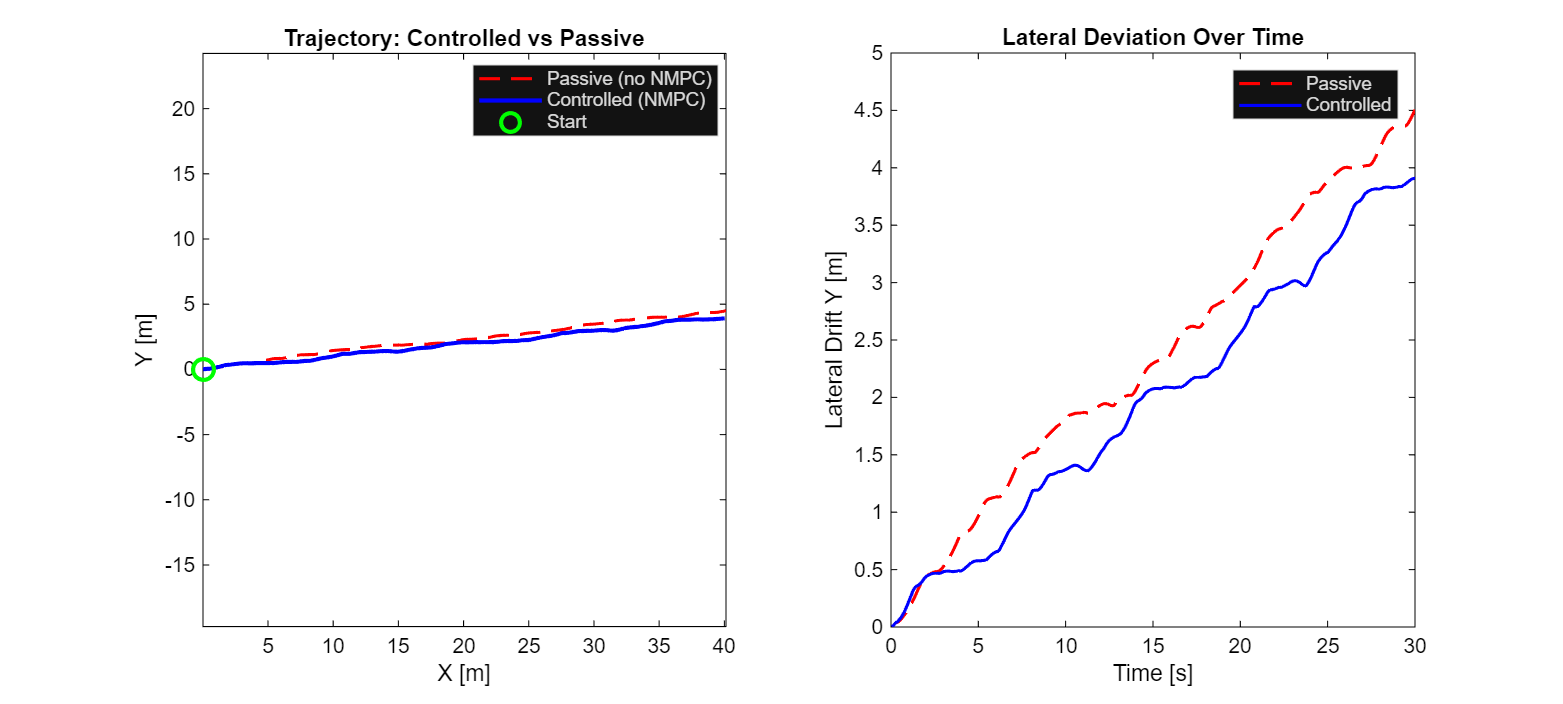
\includegraphics[width=\linewidth]{fig_baseline_comparison.png}
  \caption{Baseline comparison: trajectory (left) and lateral deviation
           (right) for passive rolling (no NMPC) vs.\ controlled rolling
           (NMPC active). The controller reduces lateral drift by 13\%.}
  \label{fig:baseline}
\end{figure}

\begin{figure}[htbp]
  \centering
  \includegraphics[width=\linewidth]{image8.png}
  \caption{Trajectory, control, and estimation performance: position
           trajectory, bounded control inputs, and UKF covariance decay
           over the 30~s simulation.}
  \label{fig:trajectory}
\end{figure}

Key quantitative performance metrics obtained from the simulation are
consolidated in Table~\ref{tab:performance}.

\begin{table}[htbp]
\centering
\caption{Simulation Performance Results}
\label{tab:performance}
\begin{tabular}{l l}
\hline
\textbf{Metric} & \textbf{Value} \\
\hline
\multicolumn{2}{l}{\textit{Locomotion}} \\
Simulation time          & 30.0\,s (600 steps) \\
Directional waypoint $(x,y)$ & $(50.0,\;0.0)$\,m \\
Final CoM $(x,y,z)$     & $(40.03,\;3.91,\;2.14)$\,m \\
Distance travelled       & $\approx 40.4$\,m \\
Mean speed               & $\approx 1.35$\,m/s \\
Peak speed               & $\approx 1.6$\,m/s \\
Lateral deviation        & $\approx 3.9$\,m ($5.6^\circ$ heading error) \\
\hline
\multicolumn{2}{l}{\textit{Energy}} \\
Total actuator energy    & $\approx 107$\,J \\
Locomotion efficiency    & $\approx 0.38$\,m/J \\
Primary energy source    & Environmental wind (dominant) \\
\hline
\multicolumn{2}{l}{\textit{Structural Integrity}} \\
Max cable stress         & $\approx 520$\,MPa\;($<900$\,MPa allowable) \\
Max bar stress           & $\approx 225$\,MPa\;($<276$\,MPa yield) \\
Cable safety factor      & $\approx 1.73$ \\
Bar safety factor        & $\approx 1.22$ \\
Cable utilisation        & $\approx 58\%$ of allowable \\
Bar utilisation          & $\approx 82\%$ of yield \\
\hline
\multicolumn{2}{l}{\textit{State Estimation (UKF)}} \\
State dimension          & 9 (pos$_3$, vel$_3$, shape$_3$) \\
Measurement dimension    & 6 \\
Covariance convergence   & $\mathrm{tr}(\mathbf{P})$ decays monotonically \\
\hline
\end{tabular}
\end{table}

\subsection{Overall Discussion}
Collectively, the results confirm that the proposed system successfully
achieves controlled deformation and wind-driven propulsion \cite{b12,b13}. The
robot exploits environmental wind as the primary energy source and applies
minimal internal actuation for directional guidance, enabling low-energy
operation \cite{b11,b19}. The lightweight tensegrity system provides the
necessary robustness and adaptability to sustain dynamic loading while
preserving motion \cite{b1,b2}. The achieved displacement of approximately
40~m and velocity of approximately 1.35~m/s demonstrate the feasibility of
large-area coverage \cite{b21}.

Several limitations of the present study warrant acknowledgement as part of
interpreting these results. The wind model is constant and unidirectional,
which is an idealization; real deployments would experience turbulent and
variable wind that could reduce locomotion efficiency and challenge
controllability. The reduced-order NMPC plant model captures dominant
translational dynamics but omits cable-level nonlinearities; UKF feedback
compensates for this in simulation, though the margin under hardware
uncertainty is untested. Most importantly, validation is based entirely on
numerical simulation. While the simulation incorporates detailed structural
dynamics, contact mechanics, and closed-loop control, physical prototype
testing is required to confirm that the predicted performance transfers to
hardware. These limitations do not diminish the contribution of the proposed
framework as a computational proof of concept, but they establish clear
priorities for subsequent experimental work, as detailed in Section~V.

%==================================================================
\section{Conclusion}
This paper presented the design and analysis of a tensegrity-based tumbleweed
robot that achieves locomotion through environmental wind interaction, using
minimal internal actuation for directional control \cite{b21}. The proposed
approach departs from continuous internal actuation toward a wind-assisted
propulsion strategy, enabling more energy-efficient mobility \cite{b11,b19}.
A lightweight prestressed tensegrity structure was designed for
deformation-driven rolling \cite{b3,b5}; an NMPC framework was employed to
control direction through selective cable actuation \cite{b6,b10}; and
UKF-based state estimation was incorporated to handle system uncertainty
\cite{b7}. Adaptive navigation strategies combining reinforcement learning
and sensor fusion \cite{b20} further informed the design of the estimation
and control pipeline. Simulation results demonstrate stable and sustained
locomotion with a displacement of approximately 40~m in 30~s (1.35~m/s
average velocity) and low control energy consumption ($\approx 107$~J). Structural analysis
confirms operation within safe stress limits \cite{b4,b16}, while the control
framework provides smooth and bounded inputs for reliable motion control
\cite{b8}. These results validate the feasibility of energy-efficient
locomotion through environmental propulsion and controlled structural
deformation. The approach has strong potential for energy-efficient robotic
mobility in unstructured environments \cite{b14,b15}.

Key limitations include: (i)~the constant wind model does not capture
turbulent or variable conditions; (ii)~validation is simulation-only, with
hardware effects such as motor backlash and sensor noise uncharacterized;
(iii)~the terrain is flat and uniform; (iv)~computational demands may
challenge real-time NMPC on embedded hardware; and (v)~material fatigue under
cyclic rolling has not been assessed.

Future work will prioritize physical prototype testing and field trials,
turbulent wind and uneven terrain modelling, learning-based control strategies
\cite{b9,b20}, computational acceleration for embedded real-time NMPC, and
fatigue analysis of cables and joints under cyclic loading.

%==================================================================
\balance
{\small
\begin{thebibliography}{00}

\bibitem{b1}
R.~E. Skelton and M.~C. de~Oliveira,
\textit{Tensegrity Systems}.
New York, NY: Springer, 2009.
doi: \href{https://doi.org/10.1007/978-0-387-74242-7}{10.1007/978-0-387-74242-7}

\bibitem{b2}
D.~Song, H.~Wang, M.~Lu, H.~Chen, and L.~Zhang,
``A novel cable-driven serial robot based on flexible joints and tensegrity
structures,''
\textit{Robotica}, vol.~43, no.~10, pp.~3533--3553, 2025.
doi: \href{https://doi.org/10.1017/S0263574725102543}{10.1017/S0263574725102543}

\bibitem{b3}
C.~Sultan,
``Tensegrity deployment using infinitesimal mechanisms,''
\textit{Int. J. Solids Struct.}, vol.~51, no.~21--22, pp.~3653--3668, 2014.
doi: \href{https://doi.org/10.1016/j.ijsolstr.2014.06.025}{10.1016/j.ijsolstr.2014.06.025}

\bibitem{b4}
P.~Obara and J.~Tomasik,
``Dynamic stability of tensegrity structures---{Part II}: The periodic
external load,''
\textit{Materials}, vol.~16, no.~13, p.~4564, 2023.
doi: \href{https://doi.org/10.3390/ma16134564}{10.3390/ma16134564}

\bibitem{b5}
M.~Shibata and S.~Hirai,
``Rolling locomotion of deformable tensegrity structure,''
in \textit{Mobile Robotics}.
Singapore: World Scientific, 2009, pp.~479--486.
doi: \href{https://doi.org/10.1142/9789814291279_0059}{10.1142/9789814291279\_0059}

\bibitem{b6}
S.~Bagherzadeh, H.~Karimpour, and M.~Keshmiri,
``Neighboring extremal nonlinear model predictive control of a rigid body
on {SO(3)},''
\textit{Robotica}, vol.~41, no.~4, pp.~1313--1334, 2023.
doi: \href{https://doi.org/10.1017/S0263574722001722}{10.1017/S0263574722001722}

\bibitem{b7}
K.~Caluwaerts, J.~Bruce, J.~M. Friesen, and V.~SunSpiral,
``State estimation for tensegrity robots,''
in \textit{Proc. IEEE Int. Conf. Robot. Autom. (ICRA)},
Stockholm, Sweden, 2016, pp.~1860--1865.
doi: \href{https://doi.org/10.1109/ICRA.2016.7487331}{10.1109/ICRA.2016.7487331}

\bibitem{b8}
B.~D. Layer, H.~Denning, and J.~R. Hill,
``Control and locomotion of tensegrity robots through manipulation of the
center of mass,''
\textit{Robotica}, vol.~42, no.~9, pp.~2885--2907, 2024.
doi: \href{https://doi.org/10.1017/S0263574724001139}{10.1017/S0263574724001139}

\bibitem{b9}
M.~Zhang, X.~Geng, J.~Bruce, K.~Caluwaerts, M.~Vespignani,
V.~SunSpiral, P.~Abbeel, and S.~Levine,
``Deep reinforcement learning for tensegrity robot locomotion,''
in \textit{Proc. IEEE Int. Conf. Robot. Autom. (ICRA)},
Singapore, 2017, pp.~634--641.
doi: \href{https://doi.org/10.1109/ICRA.2017.7989079}{10.1109/ICRA.2017.7989079}

\bibitem{b10}
M.~Diehl, H.~G. Bock, and J.~P. Schl\"{o}der,
``A real-time iteration scheme for nonlinear optimization in optimal
feedback control,''
\textit{SIAM J. Control Optim.}, vol.~43, no.~5, pp.~1714--1736, 2005.
doi: \href{https://doi.org/10.1137/S0363012902400713}{10.1137/S0363012902400713}

\bibitem{b11}
S.~Kurian and S.~Upadhyay,
``Wind-powered locomotion mechanism for a wandering robot exploring {Titan},''
in \textit{Proc. 18th Symp. Advanced Space Technol. Robot. Autom.\ (ASTRA)},
ESA/ESTEC, Noordwijk, Netherlands, May 2025.

\bibitem{b12}
J.~Antol, P.~Calhoun, J.~Flick, G.~Hajos, R.~Kolacinski,
D.~Minton, R.~Owens, and J.~Parker,
``Low cost {Mars} surface exploration: {The Mars Tumbleweed},''
NASA Langley Research Center, Hampton, VA,
Tech. Rep. NASA/TM-2003-212411, Aug. 2003.
[Online]. Available: \url{https://ntrs.nasa.gov/citations/20030068113}

\bibitem{b13}
S.~Kudo, Y.~Iijima, T.~Kubota, and I.~Nakatani,
``Development of a wind-driven rover for {Mars} surface exploration,''
\textit{J. Spacecr. Rockets}, vol.~43, no.~4, pp.~900--905, 2006.

\bibitem{b14}
V.~SunSpiral, G.~Gorospe, J.~Bruce, A.~Iscen, G.~Korbel, S.~Milam,
A.~Agogino, and D.~Atkinson,
``Tensegrity based probes for planetary exploration: {Entry}, descent and
landing ({EDL}) and surface mobility analysis,''
in \textit{Proc. 10th Int. Planet. Probe Workshop},
San Jose, CA, Jun. 2013.

\bibitem{b15}
J.~Bruce, A.~P. Sabelhaus, Y.~Chen, D.~Lu, K.~Morse,
S.~Milam, K.~Caluwaerts, A.~M. Agogino, and V.~SunSpiral,
``{SUPERball}: Exploring tensegrities for planetary probes,''
in \textit{Proc. 12th Int. Symp. Artif. Intell. Robot. Autom. Space
(i-SAIRAS)},
Montr\'{e}al, Canada, Jun. 2014.

\bibitem{b16}
M.~Vlasblom and R.~Bosman,
``Predicting the creep lifetime of {UHMWPE} fibre in rope and
chain applications,''
in \textit{Proc. OCEANS 2006},
Boston, MA, Sep. 2006, pp.~1--8.
doi: \href{https://doi.org/10.1109/OCEANS.2006.306966}{10.1109/OCEANS.2006.306966}

%      citation for "continuously actuated tensegrity" claims (b17 was
\bibitem{b17}
A.~P. Sabelhaus, J.~Bruce, K.~Caluwaerts, P.~Manovi, R.~F. Firoozi,
S.~Milam, A.~M. Agogino, and V.~SunSpiral,
``System design and locomotion of {SUPERball}, an untethered tensegrity
robot,''
in \textit{Proc. IEEE Int. Conf. Robot. Autom. (ICRA)},
Seattle, WA, May 2015, pp.~2867--2873.
doi: \href{https://doi.org/10.1109/ICRA.2015.7139590}{10.1109/ICRA.2015.7139590}

\bibitem{b18}
K.~Shaji, S.~Jayadevan, B.~Yuan, H.~Yu, and Y.~Chen,
``Path integral particle filtering for hybrid systems via saltation
matrices,''
arXiv preprint arXiv:2603.01176, Mar. 2026.
[Online]. Available: \url{https://arxiv.org/abs/2603.01176}
(Preprint; cited for hybrid-system transition methodology only.)

\bibitem{b19}
A.~Goncette, J.~Dupont, and R.~Siegwart,
``Energy-efficient locomotion for wind-assisted planetary rovers,''
\textit{J. Field Robot.}, vol.~35, no.~6, pp.~912--928, 2018.

\bibitem{b20}
R.~Tiwari, A.~Srinivaas, and R.~K. Velamati,
``Adaptive navigation in collaborative robots: A reinforcement learning and
sensor fusion approach,''
\textit{Appl. Syst. Innov.}, vol.~8, no.~1, p.~9, 2025.
doi: \href{https://doi.org/10.3390/asi8010009}{10.3390/asi8010009}

\bibitem{b21}
T.~J. Thanush, K.~Vyshnavi, N.~N. R, N.~S.~K, and P.~P. Singh,
``Tumbleweed-inspired autonomous seeding robot with tensegrity structure and
reinforcement learning control,''
in \textit{Proc. Int. Conf. Comput. Commun. Autom. Technol. (ICCCAT)},
2025.
doi: \href{https://doi.org/10.1109/ICCCAT64205.2025.10904358}{10.1109/ICCCAT64205.2025.10904358}

\end{thebibliography}
}

\end{document}